\section{Incremental User Discovery} \label{sec:Pipeline}
	
The content processing pipeline operates iteratively on a set of contexts within a given area of interest, for instance \textit{2018 UK health campaigns}. This set is initialised at the start of the process and then updated at the end of each iteration, in a semi-automated way. 
The user discovery process is therefore potentially open-ended, as long as new contexts can be discovered.
The new contexts are expected to be within the same topic area, but contexts that ``drift'' to new areas of interest are also acceptable. 
Each iteration takes a context $C$  as input, and selects a subset of the users who participate in $C$, using the topogical criteria described below, along with the  set of their features and metrics. 
These users profiles are added to a database, where entries for repeat users are updated according to a user-defined function. 
%
The pipeline structure is described below, where the numbers are with reference to Fig.~\ref{fig:twitterframework}.

\begin{figure*}
	\centering
	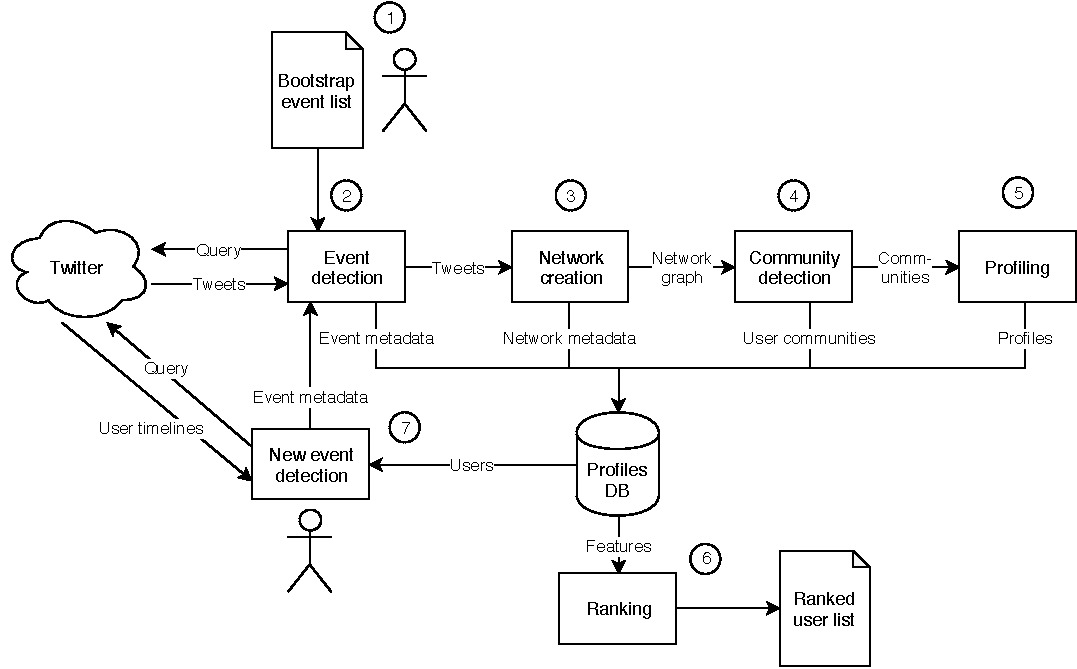
\includegraphics[width=\textwidth]{figures/TwitterFramework}
	\caption{Schematic diagram of the user discovery framework. Note that an initial list $C$ of contexts (events) is provided to initialise the \textit{event detection} step. 
	The outputs from each of these steps are persisted into the Profiles DB.}
	\label{fig:twitterframework}
\end{figure*}

%\subsection{Harvesting Content and Creating Context networks} \label{sec:harvesting}
%
Given $C$ as in (2), all Twitter posts $P(C)$ that satisfy $C$ are retrieved, using the Twitter Search APIs.
Note that this step hits the API service limitations imposed by Twitter. 
For this reason, in our evaluation we have limited our retrieval to 200 tweets/context, \anote{which is sufficient considering that repeated users do appear consistently in our evaluation (Sec.~\ref{sec:evaluation}). To overcome Twitter API limitations it can be either extended the time dedicated to harvesting (for the Twitter premium full-archive search) or choose more recent contexts as Twitter API limitations are more generous with recents tweets (for either Twitter standard search up to one week or Twitter premium 30-days search).}
%
The context network $G_C$ is then generated (3), as defined in Sec.~\ref{sec:contexts}.  %To recall, this is a directed network representing retweet and/or mention interactions between pairs of users in $C$. 
The size of each network is largely determined by the nature of the context, and  ranges between 140 and 400 users (avg 254, see Table~\ref{tab:contexts}).

%\subsection{Community detection} \label{sec:communities}

Next, $G_C$  is partitioned into communities of users (4).
The goal of this partitioning is to further narrow the scope when computing in-degree centrality (\ref{eq:IDC}), 
to enable weak-signal users to emerge relative to other more globally dominant users.
%
We have experimented with two of the many algorithms for discovering virtual communities in social networks, namely \demon~\cite{Coscia:2012:DLD:2339530.2339630} and  \infomap~\cite{INFOMAP}. 
Both are available in our implementation, but based on our experimental comparison (Sec.~\ref{sec:evaluation}) we recommend the latter.

\demon~is based on \textit{ego networks}~\cite{Arnaboldi2013}, and uses a label propagation algorithm to assign nodes to communities.  
Users may be assigned to multiple communities, an attractive feature when users are active in more than one community within the same context, i.e., a social event or a campaign.
Label propagation is also a local method, translating into an efficient algorithm.
In practice, however, in our experiments we found that for almost half of our context networks, \demon~actually fails to discover any communities.
%
In contrast, \infomap~forces each user into at most one community, but it generates valid communities in all cases. 
As some of those are very small, our  implementation discards communities with fewer than 4 users (see Sec.~\ref{sec:evaluation}).
%

%
% It has been suggested~\cite{Arnaboldi2013} that ego networks are a useful model not only to describe social relationships amongst people offline, but also the structure of their online connections. 
% Recognising that any individual may have different types of social relationships with different people (i.e., family, friends, colleagues, etc.), \demon~naturally allows for an individual to participate in multiple communities. 

% Specifically, \demon~operates on one node $v$ at a time in our context network $G_C$.

% It applies a \textit{label propagation} algorithm to each neighbour $v'$ of $v$, as follows. First, a new label $l$, which identifies a new community, is tentatively assigned to $v'$. 
% 	Then, with probability $\alpha$ $v'$ changes its label to that of the majority of its own neighbours. 
% 	At this point, each of $v$'s neighbours has a label, which is either new or that of the majority of its own neighbours (except $v$ itself).
% 	$v$ is then assigned majority labels amongst those of its neighbours. 
% 	This determines $v$'s community. 
% 	When more than one label has the same count, $v$ is assigned to all of those communities.
% %
% As a final step, communities that overlap by more than some percentage $\epsilon $ are merged.

Once communities are identified, using either method, we calculate  in-degree centrality (\ref{eq:IDC}) for each node locally, either relative to their own community if they are available, and to the entire network otherwise.

\subsection{Computing user features and ranking} \label{sec:features}

Next, user metrics as defined in Sec.~\ref{sec:metrics}, along with the \textit{Follower Rank} are computed from the network and the user features.
%
This is achieved through bulk retrieval of user profile information (5), namely the number of tweets, retweets,  number of followers $F1(u)$ and followees, $F2(u)$, along with user name, web link, and bio.
%
Computing the other metrics: \textit{Topical Focus} (\ref{eq:TF}), \textit{Topical Strength} (\ref{eq:TS}), \textit{Topical Attachment} (\ref{eq:TA}) also requires the entire user post history to be retrieved for the entire time interval defined by the context.
These posts are then separated into $P(C)$ (on-context) and $\Tilde{P}(C)$ (off-context), depending on whether they contain a hashtag related to the context or not.
Similarly, a post that contains a link is a \textit{link on-topic} if it contains both a link and a hashtag related to the context, and a \textit{link off-topic} otherwise.
We also calculate the number of retweets for every post, i.e., $\mathit{R1}(u)$ and $\mathit{R3}(u)$, which are required to compute \textit{Topical Strength}.

All of these features are persisted to a database which is made available for ranking purposes.
User-defined functions can be specified to update the Rank of pre-existing users, e.g. by combining scores assigned at different times.
%
The DB enables user-defined scoring functions, which result in user ranking lists (6). Examples of these are given later in Sec.~\ref{sec:evaluation}.
This framework approach is consistent with the experimental nature of our search for \textit{activists}, which requires exploring a variety of ranking functions.

\subsection{New contexts discovery} \label{sec:context-discovery}

The final step within one iteration (7) aims to discover new contexts, so that the process can start again (2).
Intuitively, once a score function has been applied and users have been ranked, we can hope to discover new interesting keywords and hashtags by exploring the timeline of the top-$k$ users.
Specifically,  we consider each hashtag found in the timelines, which is related to the broader topic and not yet considered in past iterations.
Each stored hashtag is then enriched with the information needed to perform a new iteration of the pipeline, namely (i) the temporal and spatial information of the context, and (ii) related hashtags.
%
Currently this step is only semi-automated, as making a judgement on the relevance of the new terms requires  human expertise.
While automating this step is not straightforward, this is not a very time-consuming step, and one can imagine an approach where such task is crowdsourced.

While the process ends naturally when no new contexts are uncovered from the previous ones, the system continuously monitors the Twitter stream for recent contexts. These may typically include events that are temporally recurring, and use similar hashtags for each new edition. In this case, their relevance is assessed on the basis of their past history.